
%(BEGIN_QUESTION)
% Copyright 2014, Tony R. Kuphaldt, released under the Creative Commons Attribution License (v 1.0)
% This means you may do almost anything with this work of mine, so long as you give me proper credit

Regn ut den største og minste spenningen som denne kretsen kan gi fra midt punktet til potensiometeret. 

$$\includegraphics[width=15.5cm]{i01131x01.eps}$$

\underbar{file i01131}
%(END_QUESTION)





%(BEGIN_ANSWER)

$U_{max}$ = 3.85 volts

\vskip 10pt

$U_{min}$ = 0.35 volts

%(END_ANSWER)





%(BEGIN_NOTES)

Be sure to ask your students how they obtained their answers, not just what the answers are.  There is more than one correct way to analyze this circuit!

Incidentally, there is nothing significant about the use of European schematic symbols in this question.  I did this simply to provide students with more exposure to this schematic convention.

%INDEX% Electronics review: series and parallel circuits

%(END_NOTES)


